\documentclass[12pt,report]{uncdissertation}
\usepackage{lmodern}
\usepackage{amssymb,amsmath}
\usepackage{ifxetex,ifluatex}
\usepackage{fixltx2e} % provides \textsubscript
\ifnum 0\ifxetex 1\fi\ifluatex 1\fi=0 % if pdftex
  \usepackage[T1]{fontenc}
  \usepackage[utf8]{inputenc}
\else % if luatex or xelatex
  \ifxetex
    \usepackage{mathspec}
  \else
    \usepackage{fontspec}
  \fi
  \defaultfontfeatures{Ligatures=TeX,Scale=MatchLowercase}
\fi
% use upquote if available, for straight quotes in verbatim environments
\IfFileExists{upquote.sty}{\usepackage{upquote}}{}
% use microtype if available
\IfFileExists{microtype.sty}{%
\usepackage{microtype}
\UseMicrotypeSet[protrusion]{basicmath} % disable protrusion for tt fonts
}{}
\usepackage[margin=1in]{geometry}
\usepackage{hyperref}
\hypersetup{unicode=true,
            pdfborder={0 0 0},
            breaklinks=true}
\urlstyle{same}  % don't use monospace font for urls
\usepackage{graphicx,grffile}
\makeatletter
\def\maxwidth{\ifdim\Gin@nat@width>\linewidth\linewidth\else\Gin@nat@width\fi}
\def\maxheight{\ifdim\Gin@nat@height>\textheight\textheight\else\Gin@nat@height\fi}
\makeatother
% Scale images if necessary, so that they will not overflow the page
% margins by default, and it is still possible to overwrite the defaults
% using explicit options in \includegraphics[width, height, ...]{}
\setkeys{Gin}{width=\maxwidth,height=\maxheight,keepaspectratio}
\IfFileExists{parskip.sty}{%
\usepackage{parskip}
}{% else
\setlength{\parindent}{0pt}
\setlength{\parskip}{6pt plus 2pt minus 1pt}
}
\setlength{\emergencystretch}{3em}  % prevent overfull lines
\providecommand{\tightlist}{%
  \setlength{\itemsep}{0pt}\setlength{\parskip}{0pt}}
\setcounter{secnumdepth}{5}
% Redefines (sub)paragraphs to behave more like sections
\ifx\paragraph\undefined\else
\let\oldparagraph\paragraph
\renewcommand{\paragraph}[1]{\oldparagraph{#1}\mbox{}}
\fi
\ifx\subparagraph\undefined\else
\let\oldsubparagraph\subparagraph
\renewcommand{\subparagraph}[1]{\oldsubparagraph{#1}\mbox{}}
\fi

%%% Use protect on footnotes to avoid problems with footnotes in titles
\let\rmarkdownfootnote\footnote%
\def\footnote{\protect\rmarkdownfootnote}

%%% Change title format to be more compact
\usepackage{titling}

% Create subtitle command for use in maketitle
\newcommand{\subtitle}[1]{
  \posttitle{
    \begin{center}\large#1\end{center}
    }
}

\setlength{\droptitle}{-2em}
  \title{}
  \pretitle{\vspace{\droptitle}}
  \posttitle{}
  \author{}
  \preauthor{}\postauthor{}
  \date{}
  \predate{}\postdate{}


%Font packages
%\usepackage[T1]{fontenc}
%\usepackage[utf8]{inputenc}
\usepackage{csquotes}
\usepackage[english]{babel}
\usepackage[utf8]{inputenc}

\DeclareUnicodeCharacter{2212}{-}

% List of acronyms
\usepackage{longtable}
%\usepackage[acronym]{glossaries}%NOTE: this will NOT work in markdown to latex. have to have access to the latex file with same name to access the glossary.

\usepackage{lscape}
\usepackage{tipa}

%% Extra packages that I added -----------------
\usepackage{textgreek}
\usepackage[table]{xcolor}
\usepackage{fancyhdr}
\usepackage{booktabs}
\usepackage{setspace}
\usepackage{kvoptions}
%\usepackage{afterpage}
\usepackage{rotating}%for sidewaystable in xtable
%\usepackage{hyperref}% to highlight links in different colors
%\hypersetup{
%    colorlinks=true,
%    linkcolor=blue,
%    filecolor=magenta,      
%    urlcolor=cyan,
%}

% see the following link for info on biblatex sort order issue: 
% http://tex.stackexchange.com/questions/51434/biblatex-citation-order
\usepackage[style=numeric,
%        hyperref=true,
        maxbibnames=99,
        firstinits=true,
        uniquename=init,
        doi=true,
%        backref=true,
        backend=biber]{biblatex}

\usepackage{float}% for placement of figures and tables

\usepackage{tikz}%for DAG
\usetikzlibrary{arrows.meta,positioning}

\usepackage{array}%for smaller landscape tables
\usepackage{graphicx}

\newcolumntype{Z}[1]{>{\raggedright\let\newline\\\arraybackslash\hspace{0pt}}m{#1}}
% \newcolumntype{C}[1]{>{\centering\let\newline\\\arraybackslash\hspace{0pt}}m{#1}}
\newcolumntype{R}[1]{>{\raggedleft\let\newline\\\arraybackslash\hspace{0pt}}m{#1}}

\usepackage{tabulary}

\usepackage[bf,singlelinecheck=off]{caption}
\usepackage{eso-pic,graphicx,transparent}% see http://stackoverflow.com/questions/32748248/watermark-in-rmarkdown

% see https://tex.stackexchange.com/questions/258688/how-to-remove-double-spacing-in-table-cell-wrap
% \usepackage{etoolbox}
% \BeforeBeginEnvironment{tabular}{\begin{singlespace}}
% \AfterEndEnvironment{tabular}{\end{singlespace}}


%%%%%%%%%%%%%%%%%%%%%%%%%%%%%%%%%%%%%%%%%%%%%%%%%%%%%%%%%%%%%
% GLOSSARIES AND ABBREVIATIONS
%%%%%%%%%%%%%%%%%%%%%%%%%%%%%%%%%%%%%%%%%%%%%%%%%%%%%%%%%%%%%
% To update the printed glossary, you need to run:
% - pdflatex dissertation
% - makeglossaries dissertation
% - pdflatex dissertation
% On Windows, you might need to install Perl first.

%% MY own note: Since I am doing this in Rmd and not LaTex need to make a separate
%% LaTex file, glossary.tex, and add the acronyms there.

%\newacronym{unc}{UNC}{The University of North Carolina at Chapel Hill}
%\makeglossaries

% NOTE: the glossaries package in LaTex does not work when using markdown. Trying another approach from "Using LaTex to Write a PhD Thesis" by Nicola L.C. Talbot



\usepackage{datagidx}% NOTE: this will not work unless you disable glossaries package

\newgidx{acronym}{{\vspace*{1\baselineskip} \normalfont\bfseries{LIST OF ABBREVIATIONS}}} % 2 line spaced after title
%\newgidx{acronym}{\large{LIST OF ABBREVIATIONS}} % 2 line spaced after title
%\DTLgidxCategorySep{1cm}

\DTLgidxSetDefaultDB{acronym}
\newacro{TC}{Total Cholesterol}
\newacro{GRS}{Genetic Risk Score}
 % has acronyms
%\input{includes/tex/glossaryfile-math.tex} % has glossaries

%\usepackage{datagidx}% NOTE: this will not work unless you disable glossaries package
%  \newgidx{glossary}{Glossary}
%  \newgidx{acronym}{List of Abbreviations}
%  
%  \DTLgidxSetDefaultDB{acronym}
%  \newacro{TC}{Total Cholesterol}
%no need to call makeglossaries.


% \newgidx{glossary}{Glossary}
% \newgidx{acronym}{List of Abbreviations}


% \DTLgidxSetDefaultDB{glossary}
% \newterm
% [%
% description={Total cholesterol},% brief description
% ]%
% {tc}% the name



%% Math Packages %%%%%%%%%%%%%%%%%%%%%%%%%%%%%%%%%%%%%%%%%%%%
\usepackage{amsmath}
\usepackage{amsthm}
\usepackage{amsfonts}
\usepackage{bbm}
\usepackage{amssymb}
\usepackage{geometry}

%% NOTE: I commented this section out. Not sure why but it kept my markdown file from compiling, kicking up a 'error 43'. Do I need to put this back? not sure.
%% Reduce spacing between paragraph and section title %%%%%%%
%% @todo: Put this modification in the class file itself.
% \usepackage{titlesec}
% \titlespacing*{\section}
% {0pt}{-5pt}{0pt}
% \titlespacing*{\subsection}
% {0pt}{-5pt}{0pt}
\usepackage{indentfirst}   %Indents first paragraphs in every section.

\setlength\parindent{24pt}

%% Flush footnotes to the left
\usepackage[hang,flushmargin]{footmisc}
%% Places footnotes immediately below horizontal rule
\setlength{\footnotesep}{0pt}

%% Normal LaTeX or pdfLaTeX? %%%%%%%%%%%%%%%%%%%%%%%%%%%%%%%%
\RequirePackage{ifpdf}

% %% Packages for Graphics & Figures %%%%%%%%%%%%%%%%%%%%%%%%%%
% \ifpdf %%Inclusion of graphics via \includegraphics{file}
% 	\usepackage[pdftex]{graphicx} %%graphics in pdfLaTeX
% \else
% 	\usepackage[dvips]{graphicx} %%graphics and normal LaTeX
% \fi


\usepackage{adjustbox}

%% EXTRA
% %%%%%%%%%%%%%%%%%%%%%%%%%%%%%%%%%%%%%%%%%%%%%%%%%%%%%%%%%%%%%%%
\usepackage{pdflscape}
\newcommand{\blandscape}{\begin{landscape}}
\newcommand{\elandscape}{\end{landscape}}

\colorlet{vlg}{gray!20}

\usepackage{tocloft}

% see https://tex.stackexchange.com/questions/4152/how-do-i-prevent-widow-orphan-lines
%\usepackage[all]{nowidow}
% Disallow all widows and orphans (clubs)
% \widowpenalty=10000
% \clubpenalty=10000
\usepackage{booktabs}
\usepackage{longtable}
\usepackage{array}
\usepackage{multirow}
\usepackage[table]{xcolor}
\usepackage{wrapfig}
\usepackage{float}
\usepackage{colortbl}
\usepackage{pdflscape}
\usepackage{tabu}
\usepackage{threeparttable}
\usepackage{threeparttablex}
\usepackage[normalem]{ulem}
\usepackage{makecell}

\begin{document}


%%%%%%%%%%%%%%%%%%%%%%%%%%%%%%%%%%%%%%%%%%%%%%%%%%%%%%%%%%%%%
%% DOCUMENT SETTINGS
%%%%%%%%%%%%%%%%%%%%%%%%%%%%%%%%%%%%%%%%%%%%%%%%%%%%%%%%%%%%%
\title{Title of dissertation}
\author{Author of dissertation}
\committee{Person 1}{Person 2}{Person 3}{Person 4}{Person 5}
\date{\today}

\abstract{The text of your abstract goes here.}	

\dedication{I dedicate this dissertation to everyone.}


\pagestyle{plain}

\frontmatter

%\maketitle% Use this command for the correct formatted version of unc dissertation page. This is adapted from the scripts written by UNC Math department graduate students. Can be found at https://github.com/mmalahe/unc-dissertation

% these are from the ..\uncdissertation.cls file
\maketitlepg
\makecopyrightpage
\makeabstractpg
\makededicationpg



% NOTE: TO DO: need to go back and make sure I have all LaTex commands I need to get spacing correction after TOC.

% The graduate school requires that entries are double spaced.
% They also require that multiple lines in a single entry are single spaced.
% This achieves that by setting \baselineskip (the space between lines)
% and \parskip (the additional space between paragraphs) directly, then restoring them
%
% @todo: Find a more elegant way of achieving this

% Establish original spacings
% 
\newlength{\oldbaselineskip}
\setlength{\oldbaselineskip}{\the\baselineskip}
\newlength{\oldparskip}
\setlength{\oldparskip}{\the\parskip}

%Set spacings for these sections
\setlength{\baselineskip}{0.5\oldbaselineskip}
\setlength{\parskip}{0.5\oldbaselineskip}


% %%%%%%%%%%%%%% START of revised code 

% Create a ``Table of Contents''
% According to template copied from http://www.cs.unc.edu/~bbb/diss/unc-dissertation-template.zip
% see frontmatter/contents.tex

\renewcommand{\contentsname}{TABLE OF CONTENTS}
\renewcommand{\cfttoctitlefont}{\textbf}
\renewcommand{\cftaftertoctitle}{\hfill}
\renewcommand{\cftdotsep}{1.5}
\cftsetrmarg{1.0in}

\setlength{\cftbeforetoctitleskip}{61pt}
\setlength{\cftaftertoctitleskip}{28pt}


% format chapter entries like other entries
\renewcommand{\cftchapfont}{\normalfont}
\renewcommand{\cftchappagefont}{\normalfont}
\renewcommand{\cftchapleader}{\cftdotfill{\cftdotsep}}

\setlength{\cftbeforechapskip}{15pt}
\setlength{\cftbeforesecskip}{10pt}
\setlength{\cftbeforesubsecskip}{10pt}
\setlength{\cftbeforesubsubsecskip}{10pt}


\clearpage
\phantomsection

% See comment at https://tex.stackexchange.com/questions/115921/wrong-numeration-in-toc-longer-then-one-page
% to fix the roman numeral numbering problem in front matter.
% Has to do with crazy compiler issue 
% NOTE: this is a really slow process so comment out next line until 100% ready to finalize document. The roman numeral lines in toc will then be correct.
\phantom{\cite{?}} 

\begin{singlespace}
\begin{center}
\tableofcontents
\end{center}
\end{singlespace}


% Create a ``List of Tables''
\renewcommand{\listtablename}{LIST OF TABLES}
\clearpage
\phantomsection
\addcontentsline{toc}{chapter}{\listtablename}

\setlength{\cftbeforelottitleskip}{-11pt}
\setlength{\cftafterlottitleskip}{22pt}
\renewcommand{\cftlottitlefont}{\hfill\textbf}
\renewcommand{\cftafterlottitle}{\hfill}

\setlength{\cftbeforetabskip}{10pt}

\begin{singlespace}
\listoftables
\end{singlespace}


% Create a ``List of Figures''

% NOTE: to add these parts to toc got this idea from https://github.com/rosannav/thesis_in_rmarkdown/tree/master/example_thesis


\renewcommand{\listfigurename}{LIST OF FIGURES}
\newpage
\phantomsection
\addcontentsline{toc}{chapter}{\listfigurename}

\setlength{\cftbeforeloftitleskip}{-11pt}
\setlength{\cftafterloftitleskip}{22pt}
\renewcommand{\cftloftitlefont}{\hfill\textbf}
\renewcommand{\cftafterloftitle}{\hfill}

\setlength{\cftbeforefigskip}{10pt}
\cftsetrmarg{1.0in}

\begin{singlespace}
\listoffigures
\end{singlespace}



% %%%%%%%%%%%%%  END of revised code  



% Restore original spacings
\setlength{\baselineskip}{1.0\oldbaselineskip}
\setlength{\parskip}{1.0\oldparskip}


\renewcommand{\listabbreviationname}{LIST OF ABBREVIATIONS}
\newpage
\phantomsection
\addcontentsline{toc}{chapter}{\listabbreviationname  }
\listofabbreviations


%\setcounter{secnumdepth}{4}
%\setcounter{tocdepth}{4}

\mainmatter

\chapter{\uppercase{Manuscript 1 --- Title here}}\addcontentsline{toc}{chapter}{\uppercase{Chapter 1: Manuscript 1 --- Title here}}

\section{Introduction}\label{introduction}

This is the introduction.

\section{Methods}\label{methods}

This is the methods section. Citation here (Knuth 2011).

\subsection{Study sample}\label{study-sample}

Put a description here with subheading.

\section{Results}\label{results}

Put some results here.

\section{Discussion}\label{discussion}

Put discussion here.

\section{Tables}\label{tables}

\singlespace

\begin{longtable}[t]{lrrr}
\caption{\label{tab:unnamed-chunk-8}Table for paper 1.}\\
\toprule
\multicolumn{1}{c}{ } & \multicolumn{2}{c}{The rest} \\
\cmidrule(l{2pt}r{2pt}){2-3}
  & column 1 & column 2 & column 3\\
\midrule
\endfirsthead
\caption[]{Table for paper 1. \textit{(continued)}}\\
\toprule
\multicolumn{1}{c}{ } & \multicolumn{2}{c}{The rest} \\
\cmidrule(l{2pt}r{2pt}){2-3}
  & column 1 & column 2 & column 3\\
\midrule
\endhead
\
\endfoot
\bottomrule
\endlastfoot
Mazda RX4 & 21.0 & 6 & 160\\
Mazda RX4 Wag & 21.0 & 6 & 160\\
Datsun 710 & 22.8 & 4 & 108\\
Hornet 4 Drive & 21.4 & 6 & 258\\
Hornet Sportabout & 18.7 & 8 & 360\\*
\end{longtable}

\blandscape

\section{Figures}\label{figures}

\begin{figure}[H]
\centering
\caption{(MS1: Figure 1) Title here.}
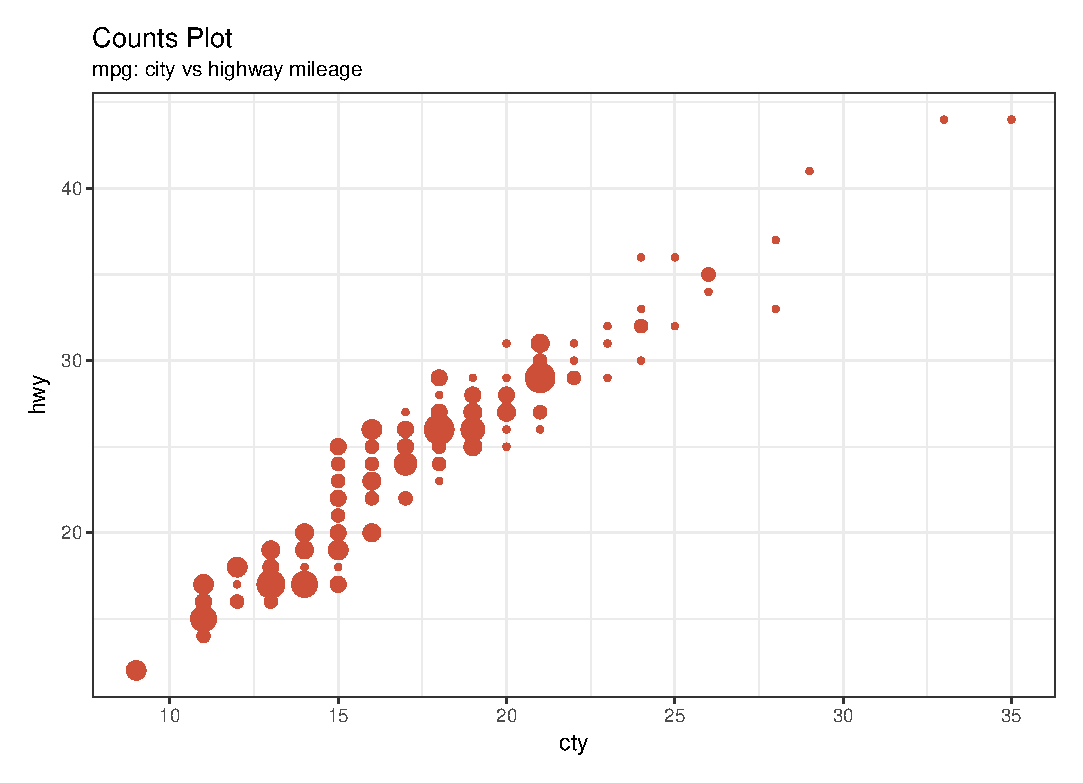
\includegraphics{includes/figures/fig1.eps}
\end{figure}

\elandscape

\chapter{\uppercase{Manuscript 2 --- Title here. Make this a very long title to demonstrate that the title is single spaced in the table of contents as required by the graduate school.}}\addcontentsline{toc}{chapter}{\uppercase{Manuscript 2 --- Title here. Make this a very long title to demonstrate that the title is single spaced in the table of contents as required by the graduate school.}}

\section{Introduction}\label{introduction-1}

This is another introduction.

Mention of a name \acr{GRS} for the first time. Mention of the acronym
for the second time, \acr{GRS}.

\section{Methods}\label{methods-1}

This is another methods section. Another citation here (Labarthe 2011).

\subsection{Study sample}\label{study-sample-1}

Put a description here with subheading.

\section{Results}\label{results-1}

Put some results here.

\section{Discussion}\label{discussion-1}

Put discussion here.

\section{Tables}\label{tables-1}

\singlespace

\begin{longtable}[t]{lrrr}
\caption{\label{tab:unnamed-chunk-11}List 1.}\\
\toprule
\multicolumn{1}{c}{ } & \multicolumn{2}{c}{The rest} \\
\cmidrule(l{2pt}r{2pt}){2-3}
  & column 1 & column 2 & column 3\\
\midrule
Mazda RX4 & 6 & 160 & 110\\
Mazda RX4 Wag & 6 & 160 & 110\\
Datsun 710 & 4 & 108 & 93\\
Hornet 4 Drive & 6 & 258 & 110\\
Hornet Sportabout & 8 & 360 & 175\\
\bottomrule
\end{longtable}

\clearpage
\newpage

\blandscape

\section{Figures}\label{figures-1}

\centering

\begin{figure}[H]
\centering
\caption{(MS2: Figure 1) Title here.}
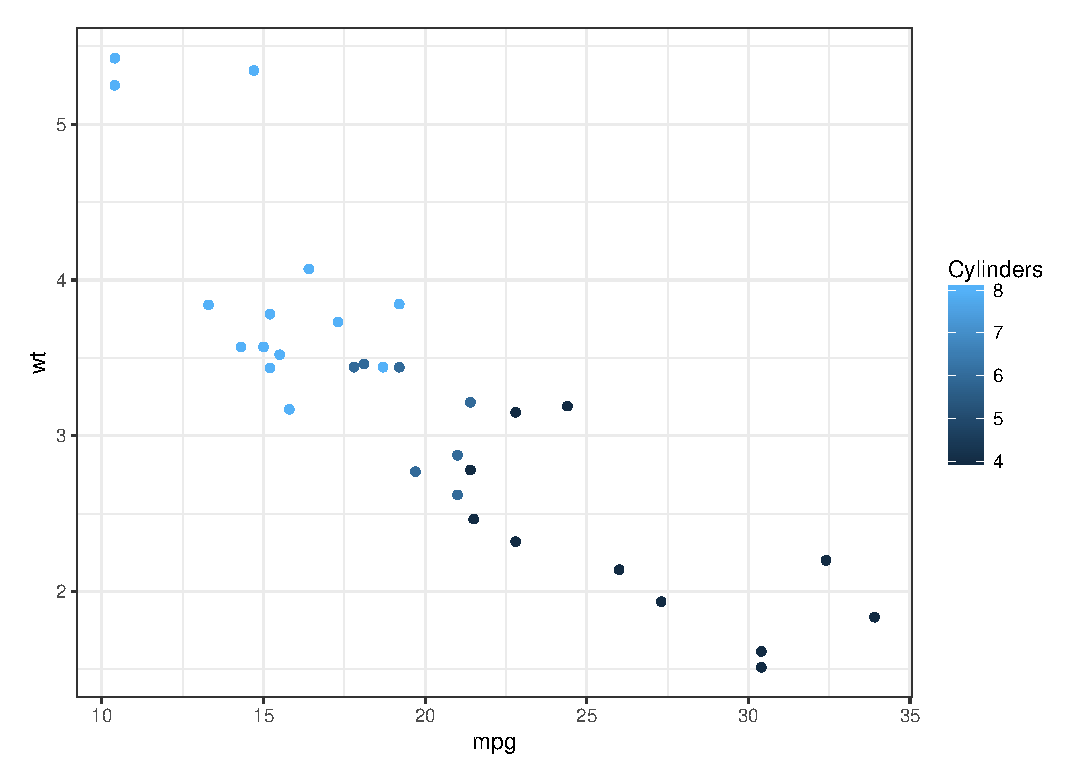
\includegraphics{includes/figures/fig2.eps}
\end{figure}

\elandscape

\setlength{\parindent}{-0.2in} \setlength{\leftskip}{0.2in}
\setlength{\parskip}{8pt}

\backmatter

\appendix

\chapter{\uppercase{Background for power calculations}}\label{app1}\addcontentsline{toc}{chapter}{\uppercase{Appendix: Useful information}}

\section{List 1}

This is one section with a formula.

\[ y = a + bx \]

\singlespace

\section{Very long title for next section that is meant to take up more than one line in the table of contents so you can verify that those lines are single spaced according to guidelines.}

\begin{longtable}[t]{lrrr}
\caption{\label{tab:unnamed-chunk-13}List 1.}\\
\toprule
\multicolumn{1}{c}{ } & \multicolumn{2}{c}{The rest} \\
\cmidrule(l{2pt}r{2pt}){2-3}
  & column 1 & column 2 & column 3\\
\midrule
\endfirsthead
\caption[]{List 1. \textit{(continued)}}\\
\toprule
\multicolumn{1}{c}{ } & \multicolumn{2}{c}{The rest} \\
\cmidrule(l{2pt}r{2pt}){2-3}
  & column 1 & column 2 & column 3\\
\midrule
\endhead
\
\endfoot
\bottomrule
\endlastfoot
Mazda RX4 & 21.0 & 6 & 160\\
Mazda RX4 Wag & 21.0 & 6 & 160\\
Datsun 710 & 22.8 & 4 & 108\\
Hornet 4 Drive & 21.4 & 6 & 258\\
Hornet Sportabout & 18.7 & 8 & 360\\*
\end{longtable}

\chapter*{REFERENCES}\addcontentsline{toc}{chapter}{REFERENCES}

\printbibliography{}

\hypertarget{refs}{}
\hypertarget{ref-knuth_mathematical_2011}{}
Knuth, Donald E. 2011. ``Mathematical Vanity Plates.'' \emph{The
Mathematical Intelligencer} 33 (1): 33--45.
doi:\href{https://doi.org/10.1007/s00283-010-9170-7}{10.1007/s00283-010-9170-7}.

\hypertarget{ref-labarthe_epidemiology_2011}{}
Labarthe, Darwin. 2011. \emph{Epidemiology and Prevention of
Cardiovascular Diseases: A Global Challenge}. 2nd ed. Sudbury, Mass:
Jones; Bartlett Publishers.


\end{document}
